\documentclass[journal]{IEEEtran}

\usepackage{amsmath,amssymb,balance,booktabs,graphicx}
\usepackage[hidelinks]{hyperref}

\graphicspath{{../../zh/figures/imagegen_20261123/}}
\newcommand{\um}{\ensuremath{\mu\mathrm{m}^{2}}}

\begin{document}
\title{FAECO: Post-Route Gate-Level ECO Area Recovery Under Time and Timing Budgets}
\author{Yalong Tong and Chang Liu%
\thanks{The authors are with the College of Computer Science and Technology, National University of Defense Technology, Changsha 410073, China (e-mail: chancews@qq.com).}}
\maketitle

\begin{abstract}
Post-route timing engineering change orders (ECOs) can increase cell area, and repeated detailed routing and timing checks limit how much of that area can be recovered within a fixed time window.
FAECO batches compatible cell substitutions under adjustable timing-loss budgets, uses relative hold failures to redirect candidate evaluation, and qualifies cumulative endpoints with detailed routing, parasitic extraction, multi-corner static timing analysis, and sequential equivalence checking.
For each batch, FAECO installs the proposed cells in a copy of the routed reference, clears the directly connected data wires, and checks the remaining geometry to identify neighboring nets that need rerouting.
On a SKY130HD Advanced Encryption Standard core, opposite-order repetitions show that this diagnosis removes one or two detailed-routing calls on the way to the same first-target physical endpoint within each scheduler.
With the same diagnosis backend and a 720\,s window, FAECO recovers 67.5648\,\um{} (0.0580\%) against 22.5216\,\um{} for original-order single-gate greedy, and reaches the common area threshold 128.37--137.84\,s earlier.
In a separate AES comparison, fixed batching reaches the threshold first and recovers 33.7824\,\um{} within the window. On an independent ASAP7 UART, the same diagnosis backend qualifies endpoints for all three schedulers, and fixed batching recovers more area than FAECO.
\end{abstract}

\begin{IEEEkeywords}
Area recovery, engineering change order, gate sizing, pre-routing diagnosis, timing budget.
\end{IEEEkeywords}

\section{Introduction}

\IEEEPARstart{P}{ost-route} timing repair changes cells and buffers after placement and routing. A timing repair engine may improve the longest paths while increasing area elsewhere~\cite{openroad}. When a design retains negative setup slack, designers may accept a bounded additional timing loss in exchange for area, provided hold, electrical limits, routing legality, and function are protected. Across eight ISCAS89 circuits, 74 of 107 individual sizing reversions leave worst negative slack (WNS) unchanged at the reporting precision under frozen parasitics. Their joint effect depends on which paths become critical and on the geometry of the revised routing.

An area-reducing substitution can retain the logical pins and still invalidate shapes near the replaced cell. Rerouting only the nets directly connected to the cell can leave an adjacent wire in conflict. A second detailed-routing call can resolve the conflict, with fewer candidates evaluated within the allotted time. The search can also spend its remaining budget splitting an early failed batch before reaching promising unvisited actions.

FAECO combines a candidate-specific pre-routing design-rule check with online scheduling and a fixed-reference acceptance policy. Independent sizing enumerates compatible substitutions from a routed netlist and cell library. Selective rollback uses upstream edit information when available. Both use physical evaluation against a frozen routed reference (Fig.~\ref{fig:framework}). Our first contribution is a pre-routing diagnosis that uses the substituted cell and remaining neighboring geometry to scope the first detailed-routing attempt. Our second contribution is a scheduler that uses relative hold failures to defer splitting and reorder unvisited actions. We evaluate the diagnosis against reactive retry within each scheduler and compare the complete search against fixed batching and original-order single-gate greedy within common time and timing budgets.

\begin{figure*}[t]
\centering
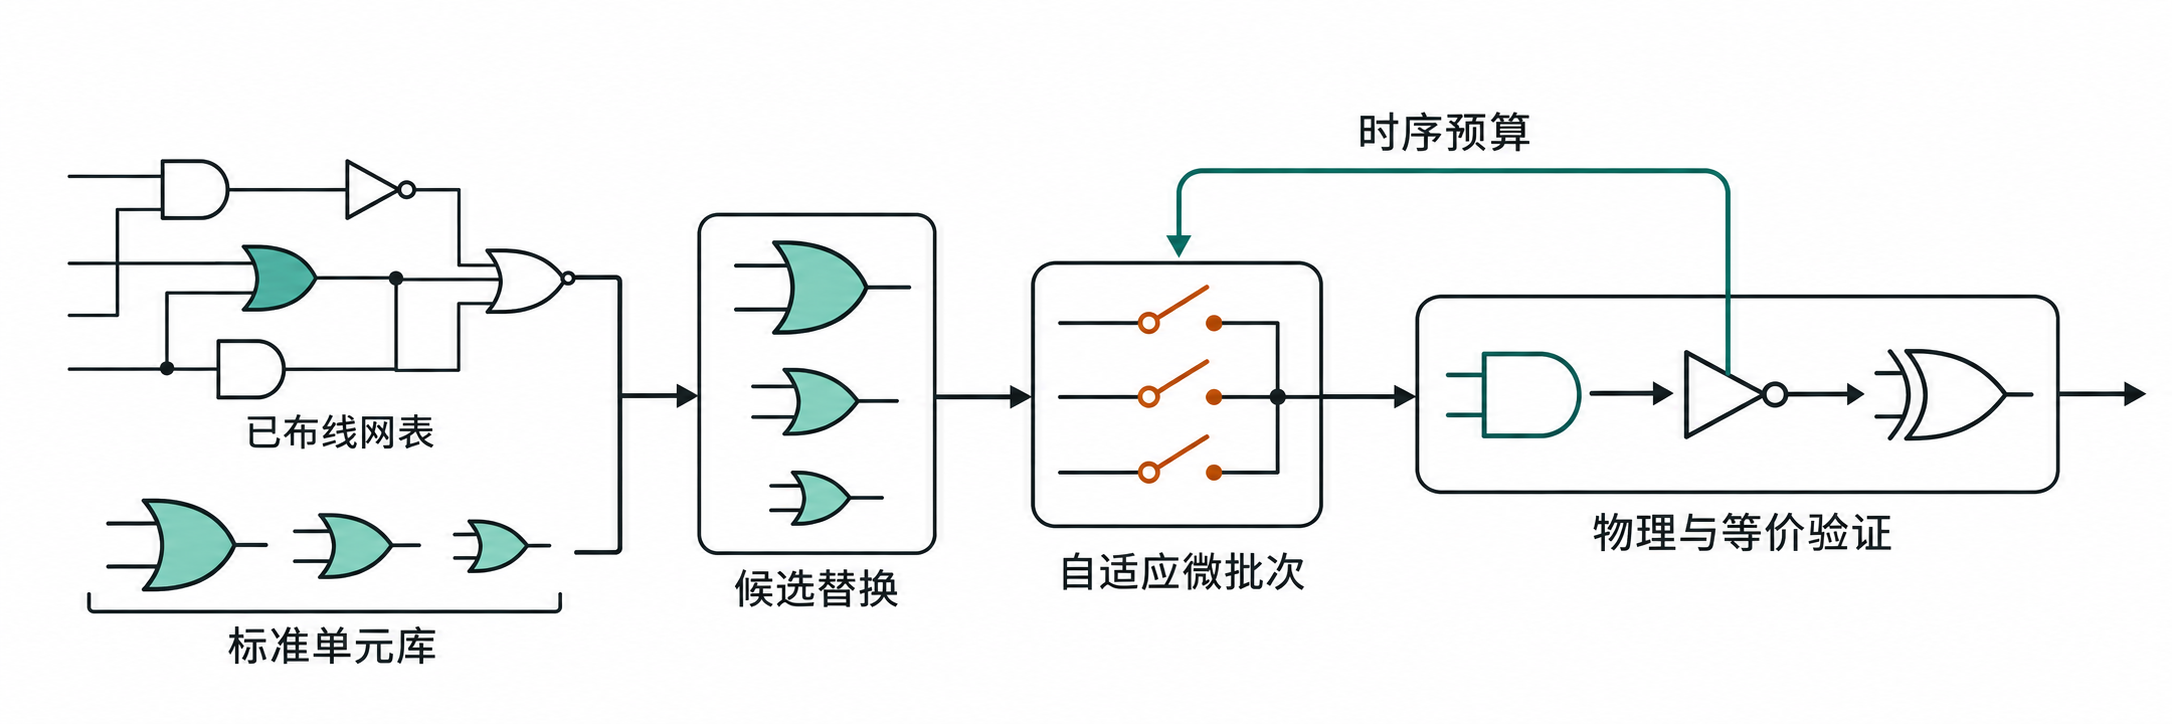
\includegraphics[width=0.94\textwidth]{01_framework.png}
\caption{FAECO workflow. The routed netlist and cell library supply candidate swaps for adaptive microbatching. Physical and equivalence checks determine acceptance, and the timing-budget gate feeds back to the scheduler.}
\label{fig:framework}
\end{figure*}

\section{Related Work}

Discrete gate sizing optimizes timing, power, and area through sensitivity ranking, Lagrangian relaxation (LR), and related methods~\cite{chen1999fast,flach2014effective,trident2}. Sizer extends sensitivity-based power reduction to industrial multi-corner multi-mode (MCMM) design and evaluates practical electrical and physical constraints~\cite{fatemi2019sizer}. FAECO measures a complementary objective, the amount of verified cell area recovered after routing within a fixed wall-clock window and a specified relative timing-loss envelope. We compare sensitivity-ranked greedy under equal evaluation counts on ten nominal endpoints and separately hold the online backend fixed in a common-wall-clock comparison with original-order greedy.

Learning-based sizers also target different stages of the optimization. DAGSizer predicts discrete reassignments from the directed timing graph to recover leakage while preserving timing~\cite{dagsizer}. LearnSize uses multipath timing and multiscale layout features to estimate the post-route timing effect of sizing changes, then optimizes sizes using gradient updates~\cite{learnsize}. FAECO's pre-routing check uses candidate geometry to determine which neighboring nets to release for physical evaluation.

TritonRoute-WXL integrates design-rule checking with detailed routing~\cite{tritonroutewxl}. CoRe-ECO jointly refines detailed placement, routing, and cell selection in windows around pin-access-related design-rule violations~\cite{coreeco}. Its evaluation concerns repairing existing violations after automatic place and route. FAECO starts from a qualified routed reference, measures conflicts introduced by a proposed area-reducing swap, and uses the reported conflicts to select neighboring signal nets to reroute. We measure how this choice affects route calls and area recovered under a time limit.

\section{Problem Formulation}

Let \(R\) denote the frozen routed reference, including the physical database, netlist, constraints, and extracted parasitics. Let \(S\) be compatible substitutions, with at most one target master per instance. For the evaluated endpoint \(N(S)\), recovered area is \(G(S)=A(R)-A(N(S))\), where \(A\) sums the areas of functional cells. The design and flow fix the library, extraction setup, and timing views \(\mathcal{V}\).

For view \(v\), let \(W_v\), \(T_v\), and \(H_v\) denote signed worst setup slack, setup total negative slack (TNS), and signed worst hold slack. We report the signed worst-slack quantities as WNS. The timed multi-corner experiments impose
\begin{align}
W_v(N(S))-W_v(R)&\geq -B_v, \label{eq:setup}\\
T_v(N(S))-T_v(R)&\geq -L_v, \label{eq:tns}\\
H_v(N(S))&\geq 0, \label{eq:absolutehold}\\
H_v(N(S))-H_v(R)&\geq -\epsilon . \label{eq:hold}
\end{align}
Here \(B_v\) and \(L_v\) are setup loss limits and \(\epsilon\) is a numerical hold tolerance. The common reference prevents allowed losses from accumulating across accepted batches. The timed experiments also require positive area recovery, zero independent design-rule and antenna violations, no additional electrical violations, and a nonempty full-netlist two-state sequential equivalence check (SEC). Setup may remain negative or cross zero under the relative policy. We report absolute slack and newly negative setup endpoints alongside relative losses. The historical nominal and explicit input/output (I/O) studies use the gates stated with their results.

The primary metric is the largest accepted \(G(S)\) by deadline \(\tau\). A second metric is the first time a fully accepted endpoint reaches a common area threshold \(G_\star\). A method that does not reach \(G_\star\) is right-censored at \(\tau\). Batches can cross the threshold by different amounts, so we report both the threshold and actual first-target areas. Fig.~\ref{fig:budget} illustrates the per-view timing budget. Wall-clock time separately limits the number of measured endpoints.

\begin{figure*}[t]
\centering
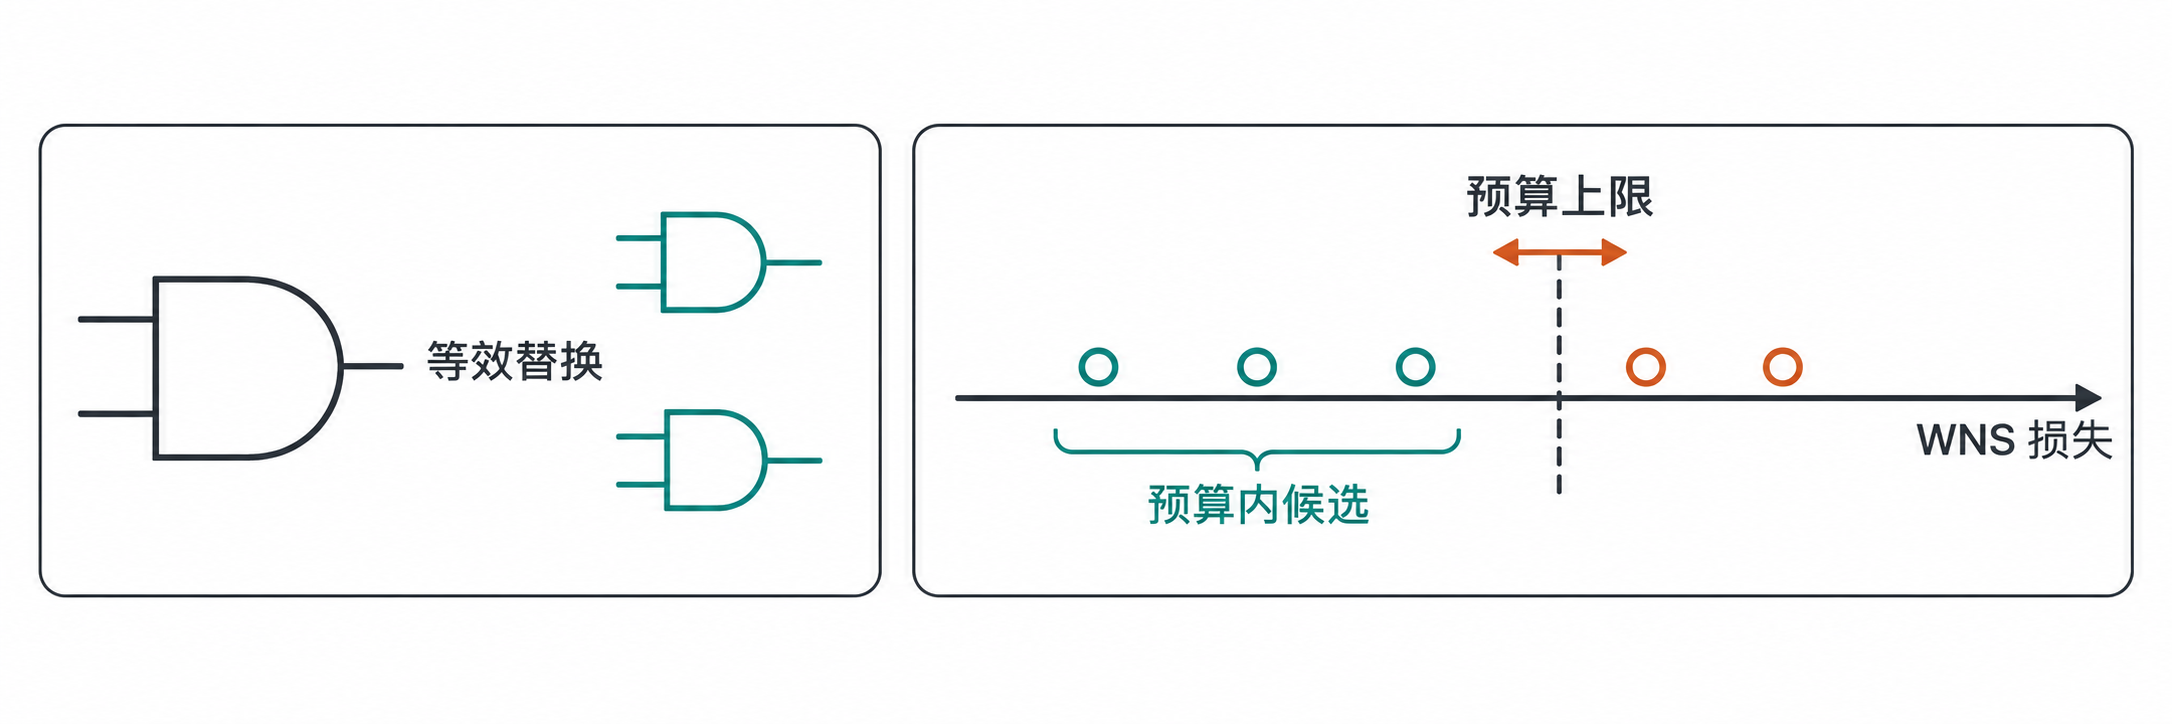
\includegraphics[width=0.92\textwidth]{02_budget.png}
\caption{Adjustable timing-loss budget. Equivalent cells provide alternative sizes. A movable WNS-loss bound determines which candidates are eligible in this view; the other endpoint checks still apply.}
\label{fig:budget}
\end{figure*}

\section{Candidate Generation and Online Validation}

\subsection{Compatible Actions and Screening}

Independent sizing enumerates compatible smaller masters from the available Liberty files and the routed netlist without requiring an upstream edit log. A substitution preserves the pin mapping and Boolean function supported by the cell models. Filler cells and dummy clock loads are excluded. Pin locations and cell widths can change even when connectivity is preserved (Fig.~\ref{fig:swap}). Fixed-parasitic timing probes can prioritize actions. Cumulative endpoints receive freshly extracted parasitics. The matched SKY130HD AES experiments begin with the same frozen order of 18 actions from the typical-corner screening step.

\begin{figure*}[t]
\centering
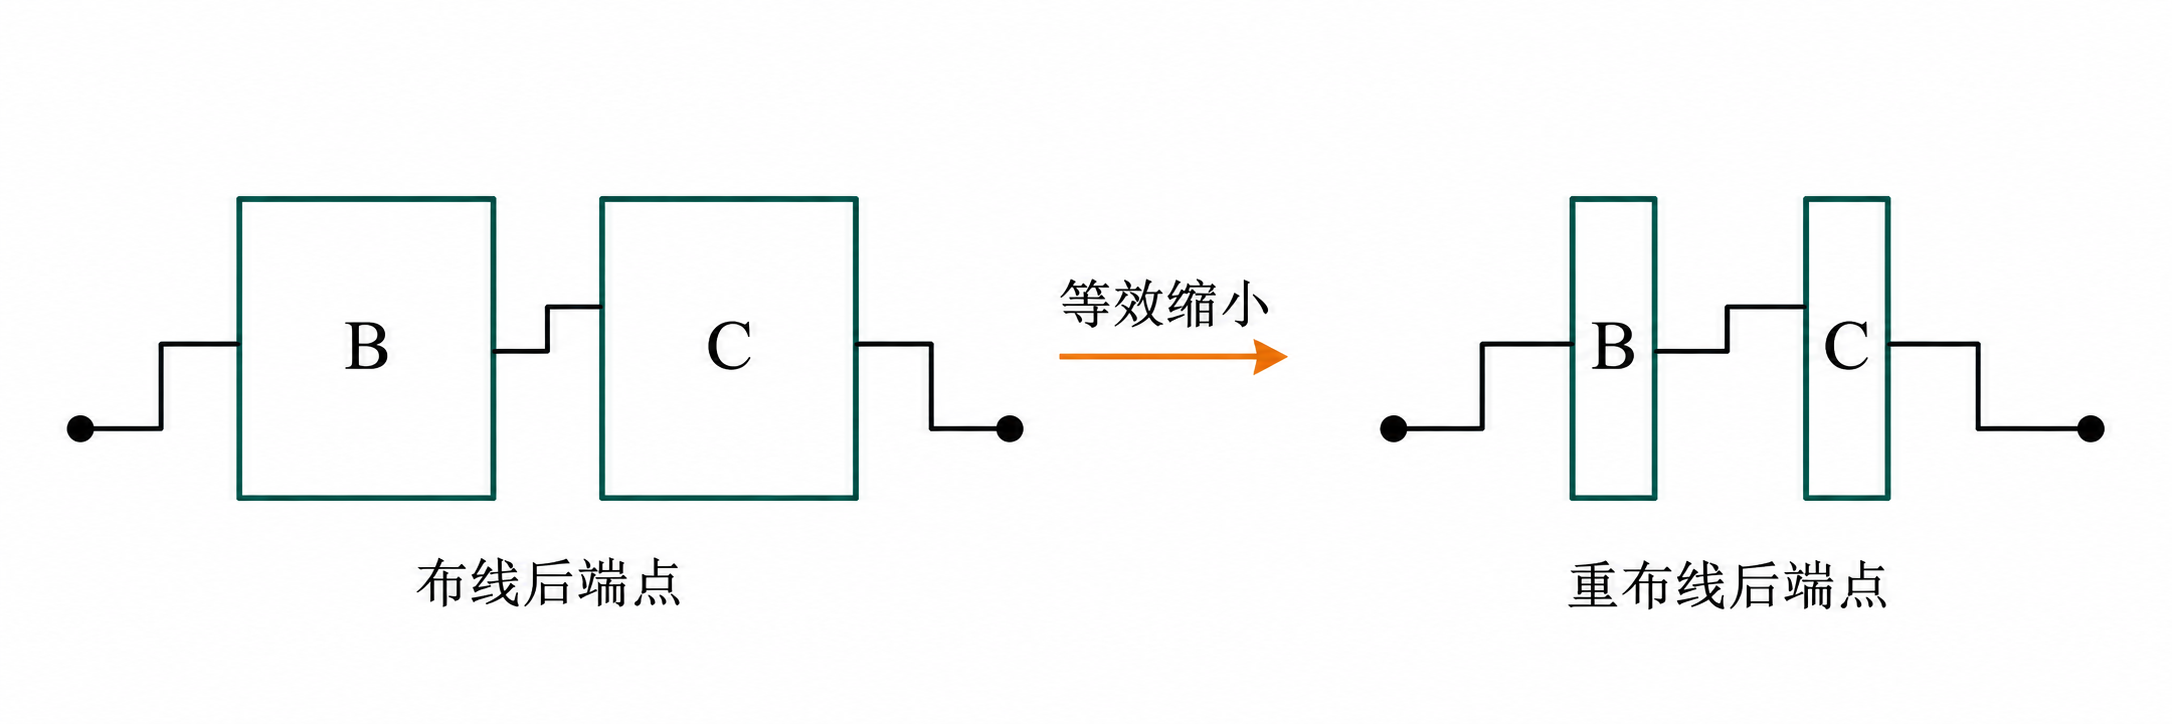
\includegraphics[width=0.89\textwidth]{05_independent_recovery.png}
\caption{Independent sizing preserves the connections. Two equivalent cells occupy less width after replacement, and wires incident to the affected pins are rerouted.}
\label{fig:swap}
\end{figure*}

Selective rollback begins with the upstream timing edits and uses individual fixed-parasitic reversions to order actions. For a failed rollback group, the search narrows the feasible-prefix boundary. It checks and retains the prefix, defers the boundary action, and retests the suffix on the accepted state (Fig.~\ref{fig:prefix}). One halving path tests \(O(\log b)\) prefixes for batch size \(b\). Nonmonotone interactions can leave useful combinations outside the tested prefixes. An online batch that expands its full subdivision tree can require \(2b-1\) evaluations.

\begin{figure*}[t]
\centering
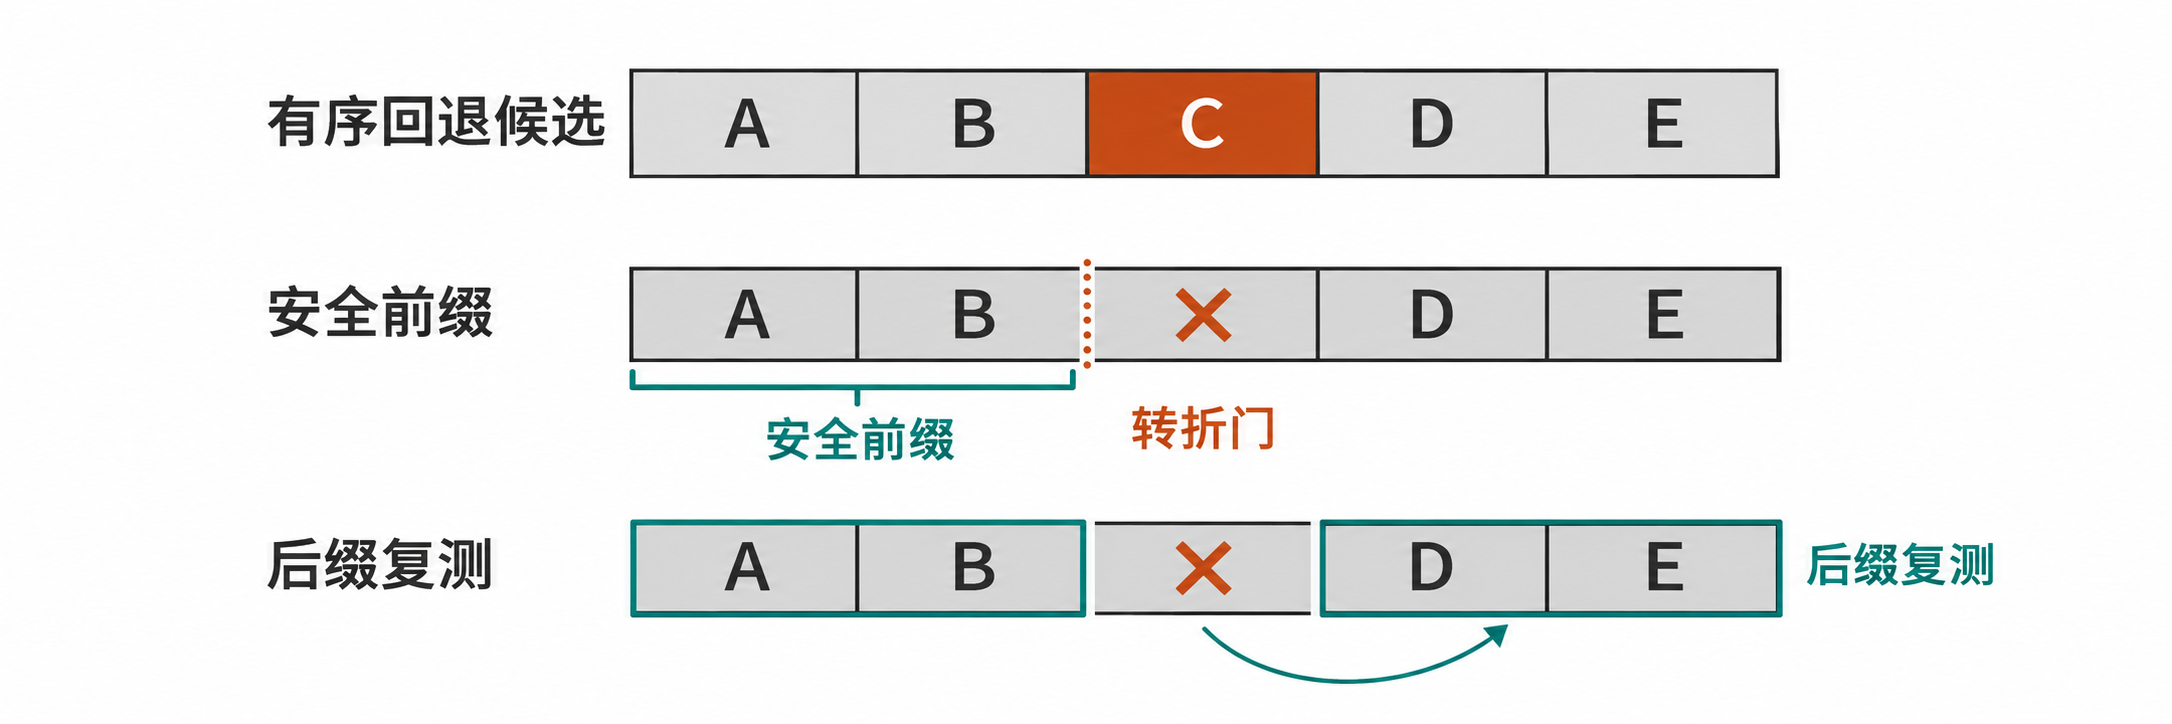
\includegraphics[width=0.92\textwidth]{03_tipping.png}
\caption{Selective rollback on ordered actions. The safe prefix is retained, the first observed boundary action is deferred, and the suffix is retested.}
\label{fig:prefix}
\end{figure*}

\subsection{Pre-Routing Conflict Diagnosis}
\label{sec:diagnosis}

Let \(\mathcal{D}(S)\) be directly connected data nets for the cumulative proposal \(S\). The backend installs the candidate cells in a copy of the frozen routed reference, removes the wires of \(\mathcal{D}(S)\), and checks the remaining shapes. If each design-rule check (DRC) marker can be attributed to a replaced instance or directly connected net and refers to at least one previously routed non-clock signal neighbor, the backend forms their union \(\mathcal{E}(S)\). It permits \(\mathcal{D}(S)\cup\mathcal{E}(S)\) to reroute on the first attempt. If the report is empty, diagnosis fails, or any marker lacks a mapping, the first attempt permits only \(\mathcal{D}(S)\). If detailed routing produces supported markers for additional neighbors, the backend can retry once with the additional nets. The reactive comparator starts with \(\mathcal{D}(S)\) and offers the same single retry from actual route markers.

Each timed local-routing evaluation applies the cumulative substitutions to the same frozen layout, protecting wires outside the permitted set. After detailed routing and resistance/capacitance extraction (RCX), the flow uses propagated-clock static timing analysis (STA), checks electrical limits by view, restores the normal routing state for independent whole-block DRC and antenna checks, and proves accepted netlists against the reference using Yosys~\cite{sta,yosys}. Fig.~\ref{fig:views} illustrates the four-view recheck used on the SKY130 benchmarks.

\begin{figure*}[t]
\centering
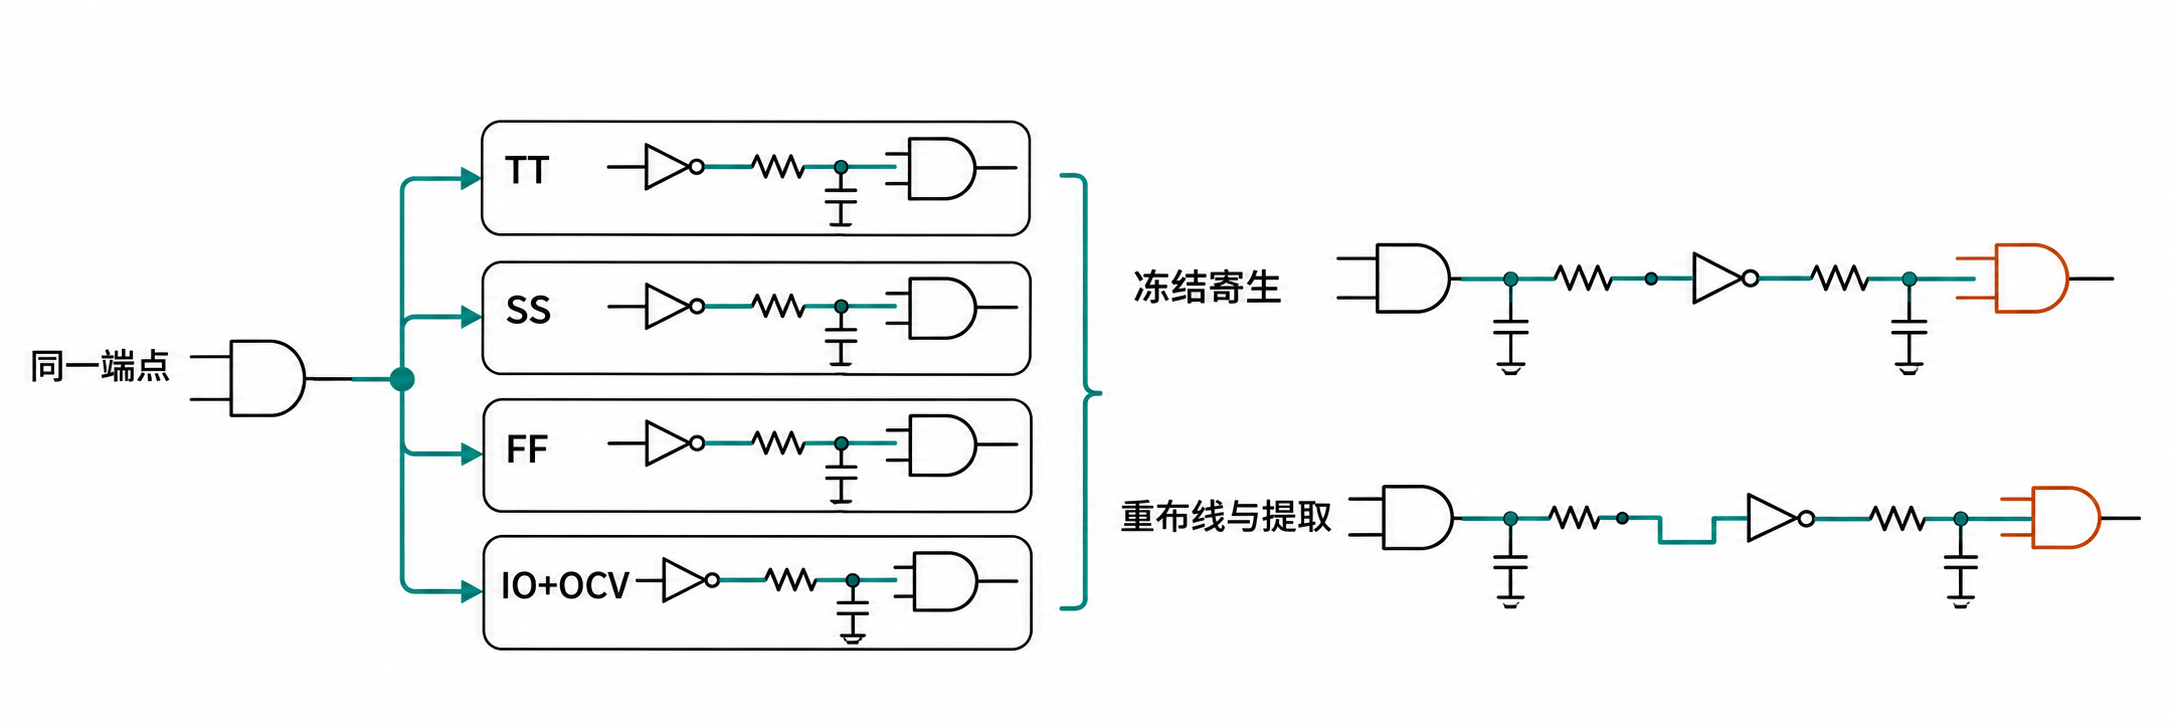
\includegraphics[width=0.92\textwidth]{04_timing_views.png}
\caption{Timing evaluation of one physical endpoint. Freshly extracted parasitics support the typical (TT), slow (SS), fast (FF), and TT I/O plus on-chip variation (OCV) views. Frozen parasitics are also used in preliminary screening.}
\label{fig:views}
\end{figure*}

\subsection{Scheduling After a Failed Batch}
\label{sec:schedule}

Original-order single-gate greedy adds one new action to the accepted set per request. Fixed batching advances through the shared initial order. FAECO evaluates batches with up to three new actions in the timed AES experiments. It commits qualifying batches and responds to a rejected multi-action batch according to the failure. If a corner fails relative hold while unvisited actions and time remain, it defers splitting that batch. On the first such deferral, it performs a stable descending sort of unvisited actions by
\begin{equation}
q_i=\frac{\Delta A_i}{1+C_i/\widetilde{C}},
\label{eq:score}
\end{equation}
where \(\Delta A_i\) is the estimated area gain and \(C_i\) sums the capacitances of the directly connected signal nets in the frozen extraction, excluding power and ground. The denominator uses the positive median \(\widetilde C\) of the candidate pool. Scores are prepared once from the frozen DEF and extracted parasitics, and preparation is charged to the timed search. This score reduces the priority of high-capacitance actions with comparable estimated area gains. Deferred batches are split in deferral order once the unvisited pool is exhausted. Other rejection reasons cause immediate bisection. A request always evaluates the new proposal together with all previously accepted actions.


\section{Evaluation}

\subsection{Protocol and Implementation}

We use OpenROAD for physical implementation and extraction, standalone OpenSTA for timing, and Yosys for two-state SEC~\cite{openroad,sta,yosys}. The wall-clock study uses a SKY130HD Advanced Encryption Standard (AES) core with its original 3.6\,ns clock period, I/O constraints, and three process, voltage, and temperature (PVT) corners. In each view \(B_v\) is 1\% of the original period (36\,ps) and \(L_v\) is the larger of 360\,ps and 1\% of \(\lvert T_v(R)\rvert\). The hold tolerance is 0.001\,ps. The target is 0.01\% of reference functional-cell area, or 11.6508\,\um. The 720\,s hard window uses the host's raw monotonic clock and charges all runs the same 113.36\,s screening cost and charges each run its actual physical evaluation, proof, retry, diagnosis, and scheduling costs. Each run can issue up to six logical requests. A request can entail a diagnosis and up to two detailed-routing calls. All arms run serially on the same host and CPU allocation, with four threads for detailed routing and one for diagnosis. For each comparison, we repeat the experiment in the reverse order.

The ten SKY130 benchmarks use a 10\,ps setup budget and fixed evaluation counts. Their nominal results, timing rechecks, and joint I/O stress tests are reported separately. The ASAP7 UART repeats the three-scheduler comparison with the same online backend under its own original constraints. Additional ASAP7 studies distinguish detailed routing and extraction from global-route parasitic estimation.

\subsection{Pre-Routing Diagnosis and Fixed-Time Recovery on AES}
\label{sec:aes}

In a six-swap development probe, checking geometry before clearing the directly connected wires returned 30 additional markers involving those old wires. After clearing them, diagnosis reported eight conflicts and four eligible neighboring nets in about 14.37\,s. The eight reported conflicts agreed with the independent DRC report after the directly connected nets had been routed in the development probe.

Table~\ref{tab:aes_factorial} crosses the reactive and diagnosis backends with fixed batching and FAECO. Each configuration has the same maximum accepted area in both orders. Within each scheduler, the two backends reach the same first-target endpoint, confirmed by matching the physical database, routed DEF, netlist, extracted parasitics after removing date metadata, and timing. For fixed batching, diagnosis eliminates one detailed-routing call before the threshold and saves 72.40--84.01\,s. For FAECO, it eliminates two calls and saves 157.95--164.38\,s. These savings include the time spent on diagnosis.

\begin{table*}[t]
\centering
\caption{SKY130HD AES factorial comparison within 720\,s. Both orders use the same 0.01\% area target and charge 113.36\,s for the shared screening.}
\label{tab:aes_factorial}
\footnotesize
\begin{tabular}{llrrrrr}
\toprule
& & \multicolumn{2}{c}{First target (s)} & \multicolumn{2}{c}{Completed requests} & Best qualified gain\\
\cmidrule(lr){3-4}\cmidrule(lr){5-6}
Scheduler & Backend & Forward & Reverse & Forward & Reverse & (\um)\\
\midrule
Fixed batching & Reactive & 448.64 & 443.27 & 3 & 3 & 33.7824\\
Fixed batching & Diagnosis & 364.63 & 370.88 & 5 & 4 & 33.7824\\
FAECO & Reactive & 641.81 & 648.25 & 3 & 3 & 33.7824\\
FAECO & Diagnosis & 483.86 & 483.87 & 4 & 4 & 67.5648\\
\bottomrule
\end{tabular}
\end{table*}

With diagnosis enabled, fixed batching reaches the shared threshold 112.99--119.23\,s earlier. FAECO subsequently accepts a six-swap endpoint at 619.31 and 620.07\,s, doubling the fixed-batch gain within the window. With the reactive backend, both schedulers recover 33.7824\,\um. A fifth, nine-swap FAECO request is cut off during timing analysis in both factorial runs. Separate development qualification of the same proposal measures 98.8448\,\um{} of recovery and one new negative TT setup endpoint under the allowed setup budget. The result is outside the timed comparison.

The six-swap endpoint improves hold WNS in all three corners and loses at most 0.086\,ps of setup WNS. It creates no new negative setup endpoints. Table~\ref{tab:aes_greedy_timing} gives its per-corner timing changes. Only 22 allowed data nets change route geometry, and the 15,635 protected nets retain their geometry. Independent DRC and antenna counts are both zero. SEC proves 11,089 points with zero unproven points.

\subsection{A Matched Online Comparison with Single-Gate Greedy}

In a separate timed experiment, original-order single-gate greedy and FAECO share the diagnosis backend, the initial action pool, the 720\,s hard window, and the same acceptance gates. Table~\ref{tab:aes_greedy} reports the opposite-order repetitions. Both schedulers complete four of five issued requests and accept two checkpoints per order. FAECO tests 12 distinct new actions within its four completed requests, and greedy tests four. FAECO advances by three actions per accepted batch, while greedy adds one action per acceptance.

\begin{table}[t]
\centering
\caption{SKY130HD AES matched online comparison. Both schedulers use diagnosis and the same initial candidate order.}
\label{tab:aes_greedy}
\footnotesize
\begin{tabular}{lrrr}
\toprule
& \multicolumn{2}{c}{First target (s)} & Best gain\\
\cmidrule(lr){2-3}
Scheduler & Forward & Reverse & (\um)\\
\midrule
Single-gate greedy & 607.81 & 599.80 & 22.5216\\
FAECO & 469.96 & 471.42 & 67.5648\\
\bottomrule
\end{tabular}
\end{table}

At a common threshold of 11.6508\,\um, FAECO qualifies 33.7824\,\um{} on its first accepted endpoint, and greedy qualifies 22.5216\,\um{} on its second. Greedy first qualifies a single swap for 11.2608\,\um{} at 357.14--361.03\,s, earlier than FAECO's first accepted endpoint and slightly below the common area threshold. FAECO rejects its initial batch on SS relative hold. One action from that batch passes by itself in greedy. A subsequent greedy addition fails on SS hold, while FAECO uses that type of failure to move on to other batches.

Both best endpoints have zero independent DRC and antenna violations, meet the hold and electrical gates, and prove 11,089 equivalence points each. No new negative setup endpoints appear. Table~\ref{tab:aes_greedy_timing} reports the timing tradeoff. The greatest setup WNS loss is below 0.1\,ps for both endpoints. At SS, greedy improves setup TNS while FAECO incurs a loss within the budget. FAECO's six-swap endpoint matches the one accepted in the factorial experiment. This comparison measures the combined effect of batching, rejection handling, and subsequent order changes.

\begin{table}[t]
\centering
\caption{AES timing changes at the best qualified endpoints in the matched online comparison (ps).}
\label{tab:aes_greedy_timing}
\footnotesize
\setlength{\tabcolsep}{2.5pt}
\begin{tabular}{lrrrr}
\toprule
& \multicolumn{2}{c}{\(\Delta\) setup/hold WNS} & \multicolumn{2}{c}{\(\Delta\) setup TNS}\\
\cmidrule(lr){2-3}\cmidrule(lr){4-5}
View & Greedy & FAECO & Greedy & FAECO\\
\midrule
FF & \(-0.0058/+0.0001\) & \(-0.0857/+0.0490\) & \(0\) & \(0\)\\
TT & \(-0.0262/+0.0004\) & \(-0.0320/+0.0768\) & \(-2.685\) & \(+10.244\)\\
SS & \(-0.0053/+0.0526\) & \(-0.0435/+0.7303\) & \(+105.274\) & \(-192.358\)\\
\bottomrule
\end{tabular}
\end{table}

\subsection{Nominal Recovery and Four-View Endpoint Rechecks}

On ten SKY130 circuits, independent sizing under the nominal 10\,ps setup WNS budget and a relative hold gate recovers 0.67\%--5.58\% of total cell area in 6--10 physical evaluations per circuit. These six ISCAS89 and four ITC-99 endpoints all pass DRC and full-netlist two-state SEC. Table~\ref{tab:aligned} aligns those same netlists and corresponding fresh parasitics with four timing views. The nominal selection and later rechecks use their respective bound physical references.

\begin{table*}[t]
\centering
\caption{Same-endpoint SKY130 rechecks. Timing columns report paired setup/hold WNS changes (ps) relative to each view's reference. The last column gives absolute I/O+OCV hold WNS for reference and candidate.}
\label{tab:aligned}
\footnotesize
\begin{tabular}{lrrrrrr}
\toprule
Circuit & Area recovery & TT & SS & FF & TT I/O+OCV & I/O+OCV hold\\
\midrule
s382 & 1.78\% & \(-6.705/0.000\) & \(+34.940/0.000\) & \(+1.724/0.000\) & \(+15.465/-0.059\) & \(-100.759/-100.819\)\\
s420 & 5.58\% & \(+4.120/+0.013\) & \(+17.917/+0.074\) & \(-2.840/+0.014\) & \(+5.732/+0.689\) & \(-67.435/-66.746\)\\
s641 & 1.99\% & \(-0.427/+0.104\) & \(-18.505/+0.791\) & \(+2.104/-1.400\) & \(+4.907/-0.362\) & \(-82.559/-82.921\)\\
s713 & 2.32\% & \(+0.629/+3.646\) & \(-4.583/+41.831\) & \(+0.404/-3.944\) & \(-10.147/+0.197\) & \(-98.312/-98.116\)\\
s832 & 1.71\% & \(-4.165/+2.643\) & \(+40.008/+4.722\) & \(-5.409/+2.053\) & \(-17.204/+0.156\) & \(-74.680/-74.524\)\\
s953 & 0.67\% & \(-9.880/+2.988\) & \(+90.459/+7.789\) & \(+2.310/+2.038\) & \(-7.108/-1.027\) & \(-118.625/-119.652\)\\
b04 & 0.86\% & \(+5.311/+0.070\) & \(+53.423/-0.130\) & \(+3.409/-0.102\) & \(+5.961/+3.197\) & \(-123.293/-120.096\)\\
b05 & 3.47\% & \(+6.706/+1.894\) & \(+20.826/-2.327\) & \(+3.779/-1.383\) & \(+3.834/+2.829\) & \(-41.337/-38.507\)\\
b11 & 0.90\% & \(+4.989/-1.632\) & \(+20.655/-0.467\) & \(-29.022/-0.177\) & \(+5.225/+0.473\) & \(-81.881/-81.408\)\\
b12 & 0.82\% & \(+1.441/+0.089\) & \(+64.588/+0.306\) & \(+29.798/+0.066\) & \(+1.461/-4.932\) & \(-40.949/-45.881\)\\
\bottomrule
\end{tabular}

\smallskip
\parbox{0.95\textwidth}{\footnotesize An independently rerouted reference is used in all four views for s420, s641, s713, s832, and s953. The I/O+OCV reference for b05 is independently rerouted. The other references are the corresponding original Resizer endpoints.}
\end{table*}

The TT, SS, and FF libraries use \(25\,^\circ\mathrm{C}\) at 1.80\,V, \(-40\,^\circ\mathrm{C}\) at 1.40\,V, and \(-40\,^\circ\mathrm{C}\) at 1.95\,V, respectively. The separate TT I/O+OCV view imposes 0.10\,ns input and output delays, 0.01\,pF output load, 0.05\,ns input transition, and early/late derates of 0.90/1.10. Nine of ten aligned endpoints meet the 10\,ps SS setup budget. Five of ten retain FF hold WNS. The 10\,ps I/O+OCV setup gate passes eight endpoints, with s713 and s832 exceeding the loss bound. All ten candidates and their corresponding I/O+OCV references have negative absolute hold WNS. A different s641 endpoint recovers 0.66\% and passes SS setup, FF relative hold, and SEC. Its I/O+OCV result was not measured. Its historical TT pair used different library revisions.

\subsection{Joint-Gate Searches on s713 and s832}

For each circuit we freeze a single Resizer layout and test ten candidates plus a zero-swap reroute. All four views use the same endpoint netlist and corresponding extracted parasitics. Positive recovery requires zero DRC, no more than 10\,ps of setup WNS loss in any view, and both nonnegative absolute and nondegrading relative hold in all four views. The original 0.5\,ns propagated clock is used with a 0.001\,ps relative hold tolerance. TNS is recorded for diagnosis. All twenty candidates pass DRC. I/O+OCV hold WNS is \(-98.219\) and \(-75.316\)\,ps for the original s713 and s832 references and remains negative for both zero-swap reroutes and all twenty candidates. Neither circuit achieves positive recovery under the joint gate.

With just absolute I/O+OCV hold relaxed for diagnosis, s713 still yields zero qualified recovery. An s832 endpoint saves 3.7536\,\um{} (0.322\%) and improves I/O+OCV setup and hold WNS by 6.404 and 0.801\,ps, respectively. Its absolute I/O+OCV hold WNS remains \(-74.515\)\,ps. SEC proves 162 points with none unproven.

\subsection{Historical Nominal Baselines and Power}

Fig.~\ref{fig:compare} shows the five comparison arms. Native OpenROAD recovery follows its built-in policy. Frozen-parasitic sensitivity batching and a five-round frozen-parasitic LR implementation select an endpoint offline for physical re-evaluation. Online sensitivity-ranked single-gate greedy and historical FAECO share a limit of 6--10 rerouted evaluations per circuit. All use the same corresponding physical starting inputs and a 10\,ps nominal setup WNS loss limit for endpoint assessment. Native recovery makes no substitutions on this SKY130 set. Its different behavior on the ASAP7 AES case is reported below.

\begin{figure*}[t]
\centering
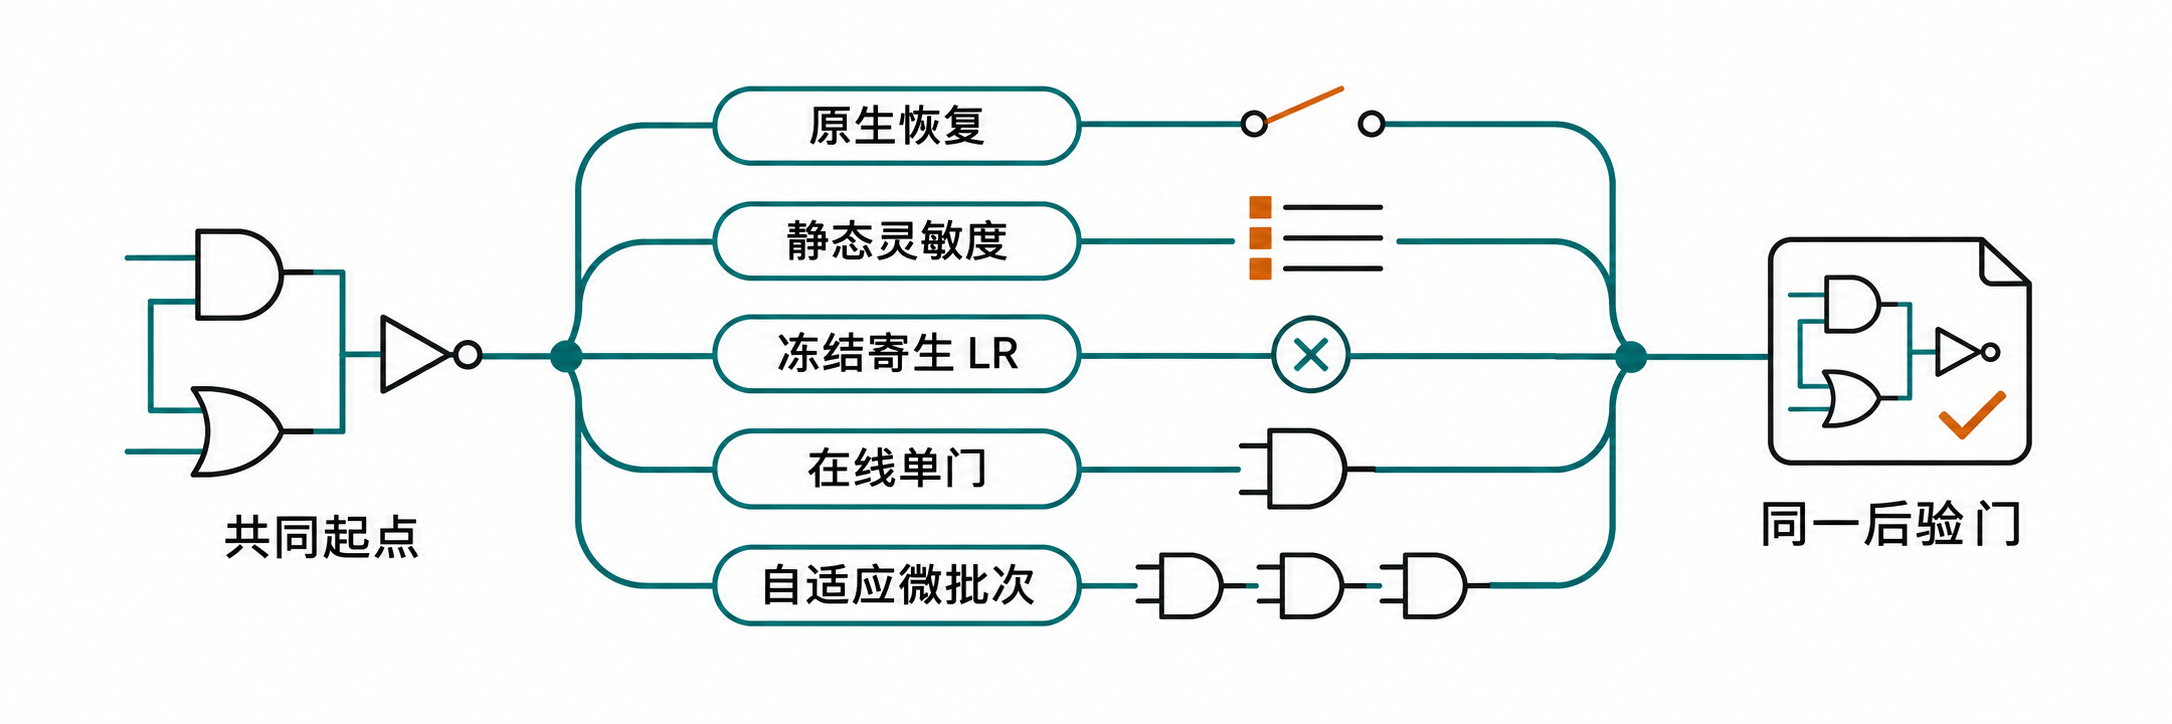
\includegraphics[width=0.92\textwidth]{06_comparison.png}
\caption{Five nominal comparison arms from one routed reference. The lanes are native recovery, frozen-parasitic sensitivity, frozen-parasitic LR, online single-gate greedy, and adaptive microbatching. Reported endpoints face the same physical assessment.}
\label{fig:compare}
\end{figure*}

\begin{table}[t]
\centering
\caption{Qualified area reduction in the ten-circuit nominal comparison. Means include zero-recovery circuits.}
\label{tab:nominal_baselines}
\footnotesize
\begin{tabular}{lrr}
\toprule
Method & Positive endpoints & Mean recovery\\
\midrule
OpenROAD native recovery & 0/10 & 0.00\%\\
Frozen-parasitic sensitivity batch & 5/10 & 0.14\%\\
Frozen-parasitic LR & 0/10 & 0.00\%\\
Online sensitivity-ranked greedy & 9/10 & 2.11\%\\
Historical FAECO & 10/10 & 2.01\%\\
\bottomrule
\end{tabular}
\end{table}

As shown in Table~\ref{tab:nominal_baselines}, each online method recovers more area on five circuits. On s713 the same three-action endpoint arrives on request four with sensitivity order and request eight with the original order. On s953 original area order accepts a 0.67\% saving on its first action, which is outside the first six sensitivity-ranked requests. On b12 both action order and batch size change, with FAECO recovering 0.82\% and greedy 0.41\%. Four historical FAECO endpoints in this set use one-action increments. The comparison therefore measures the complete strategies under the nominal protocol.

The frozen-parasitic LR implementation proposes 7.81\%--14.14\% area reduction offline. Its ten endpoints lose 79.60--706.03\,ps of setup WNS after physical re-evaluation and exceed the allowed loss. Power reports for the FAECO nominal endpoints show a mean decrease of 0.96\% in total power and 3.72\% in combinational power relative to the corresponding references.


\subsection{Selective Rollback and Regional Routing}

A fixed pool of 52 routed s382 endpoints yields 6, 15, 19, and 21 eligible endpoints with WNS loss budgets of 0, 5, 10, and 20\,ps, respectively. The best certified area recovery is 0.59\% at 0\,ps and 4.40\% at each larger budget. The latter recovers 28.91\% of the net area added by Resizer, loses 3.098\,ps of setup WNS and 231.982\,ps of TNS, improves hold WNS by 3.577\,ps, and proves 101 equivalence points. These values come from re-screening the fixed physical pool. In online greedy and bounded-beam tests with up to 12 evaluations, greedy recovers 22.52\,\um{} versus 15.01\,\um{} on s641, and both recover 16.27\,\um{} on s953 under the strict relative hold gate.

In a frozen-parasitic selective rollback study of 16 ITC-99 circuits, 15 had upstream edits. The search reverts 857 of 971 actions and recovers 27.8\% of aggregate net added area. Jointly reverting all 359 actions on b22 loses 106.4\,ps of setup WNS even though its single reversions are flat at the reporting precision. Linear rollback reaches the 600\,s limit at its 143rd evaluation. Prefix search and suffix retesting use 10 STA evaluations to recover 356 edits, demonstrating the effect of retaining a critical action for this fixed-parasitic case.

On b12, local routing for the same candidate completes in 52.94\,s with 16 remaining DRC violations. Full reroute takes 112.02\,s and passes DRC. On b15, full-die reroute still has 66 violations after 1426.14\,s. Six local incremental evaluations finish with zero DRC in 184.83--200.92\,s per evaluation. The accepted five-swap endpoint recovers 88.84\,\um{} (0.26\%) and passes two-state SEC. Its TT hold WNS decreases by 0.021\,ps within the registered 0.05\,ps extraction tolerance. On b14, the compatible downsizing pool is empty because supported combinational cells are already at minimum drive.

\subsection{ASAP7 and Additional Original-Constraint Starting Points}

On ASAP7 Ibex, an earlier scheduler comparison uses original I/O constraints, a per-view 10\,ps setup WNS loss envelope, TNS loss limits, and the same hold, electrical, DRC, and SEC gates across arms. Both schedulers reach the 0.01\% area target on their third detailed-routing and extraction call in both run orders. They qualify the same two-swap endpoint for 0.26244\,\um{} (0.012322\%) and prove 17,363 equivalence points. FAECO saves 35.20--40.31\,s on the WSL monotonic clock, primarily through one fewer intermediate SEC. The detailed-routing and extraction time differences change direction across orders. FF setup WNS crosses from \(+0.380\) to \(-4.380\)\,ps and adds 15 negative setup endpoints under the allowed relative budget. Shared start and zero-swap qualification are charged separately. A separate six-call comparison on the same benchmark found 0.37908\,\um{} for single-gate greedy and 0.26244\,\um{} for FAECO; both recovered 0.26244\,\um{} at the 1325.60\,s common cutoff.

A separate ASAP7 AES experiment estimates parasitics from global routing with ideal clocks. Its common starting setup WNS is \(-85.28\)\,ps. Native recovery reduces area by 0.118\% and worsens setup TNS by 2516.01\,ps. FAECO reduces area by 0.266\%, leaves reported setup and hold WNS unchanged, and improves TNS by 48.18\,ps. These runs use different evaluation budgets and a different physical stage from the SKY130HD detailed-route comparison.

SKY130HD JPEG completes detailed routing and extraction under its original 5\,ns clock and I/O constraints. Its starting SS hold WNS is \(-2.341\)\,ns, excluding it from the candidate comparison under the absolute hold gate.

\subsection{Transfer to ASAP7 UART Under Original Constraints}
\label{sec:uart}

The ASAP7 universal asynchronous receiver-transmitter (UART) starts from a natively routed and extracted design under its original 270\,ps period, 54\,ps I/O delays, and 66.270\,ps virtual clock latency. Its FF/TT/SS hold WNS values are \(+50.315/+67.502/+54.053\)\,ps. TT and SS setup already have negative endpoints. Independent DRC and antenna counts are zero, electrical limits pass, and the starting netlist self-SEC proves 567 points. A shared zero-swap evaluation also passes the full gate and preserves the original netlist. Its time is recorded separately.

We use the same online diagnosis and protected routing backend for original-order greedy, fixed batching, and FAECO in forward and reverse orders. The 720\,s window charges each run 81.56\,s of common pre-screening. It admits up to six requests from the same 18-action pool, and batching starts with three new actions. Each corner may lose up to 2.7\,ps of setup WNS. FF/TT/SS setup TNS loss limits are 27/27/136.974\,ps. The absolute and relative hold, electrical, DRC, antenna, and two-state SEC checks remain active. The 0.01\% area target is 0.0079009\,\um{} of the reference's 79.00902\,\um{} of functional-cell area.

\begin{table}[t]
\centering
\caption{ASAP7 UART matched online comparison under original constraints.}
\label{tab:uart}
\footnotesize
\begin{tabular}{lrrr}
\toprule
& \multicolumn{2}{c}{First target (s)} & Best gain\\
\cmidrule(lr){2-3}
Scheduler & Forward & Reverse & (\um)\\
\midrule
Single-gate greedy & 152.16 & 151.16 & 0.17496\\
Fixed batching & 152.78 & 152.07 & 0.23328\\
FAECO & 151.80 & 152.29 & 0.14580\\
\bottomrule
\end{tabular}
\end{table}

All six runs complete six requests before the deadline. Table~\ref{tab:uart} shows that fixed batching recovers the most area in both orders, followed by single-gate greedy and FAECO. First-target times span 151.16--152.78\,s across all six runs, with a different fastest scheduler in each order. Actual gains at the first accepted endpoint are 0.08748\,\um{} for single-gate greedy and FAECO and 0.17496\,\um{} for fixed batching. The comparison verifies that the online backend can apply the diagnosis and qualify area-reducing endpoints on another technology. The scheduling advantage seen on SKY130HD AES does not recur here.

In both FAECO orders, requests two and four evaluate the same cumulative three actions, with matching routed database, DEF, and netlist. Both fail the FF setup-loss gate. Accepting a singleton during the split makes it possible for the next suffix request to reconstruct the parent proposal from the frozen start. The repeated proposal takes 19.57 and 19.54\,s for physical evaluation, or 23.22 and 23.32\,s including diagnosis, in forward and reverse order. It uses one of the six request slots in each run.

\section{Discussion}

The fixed-scheduler backend comparisons on SKY130HD AES identify fewer route calls with matched physical endpoints. The scheduler comparisons expose a separate tradeoff. Greedy returns the first small accepted gain, fixed batching reaches the study's common area threshold earliest in its paired experiment, and FAECO achieves greater in-window recovery. The scheduler jointly changes candidate coverage and cost. On ASAP7 UART, the same backend qualifies smaller gains for FAECO than for the two comparators, with one of six requests consumed by a repeated cumulative proposal. The frozen-reference identity provides a direct criterion for detecting such repeats. Separating order, batch width, and response to failure requires controlled comparisons under the same backend.

Candidate order can concentrate timing risk. In the SKY130HD Ibex comparison without screening, the worst TT setup paths of all 18 candidates traverse a high-fanout buffer downsized from \texttt{buf\_12} to \texttt{buf\_1}. Applying the swapped cells with reference parasitics loses 474.64 and 403.73\,ps of setup WNS on two representative candidates. Replacing only the parasitics shifts WNS by less than 1\,ps on either candidate. This identifies drive loss in those cases and motivates screening before detailed routing. In an earlier screened controller matrix, repeated splitting restricted FAECO to the top four candidates in six calls; fixed batches reached lower-ranked feasible groups on Ibex and GCD. Hold-triggered deferral addresses this observed coverage pattern, and the newer comparison on AES also changes the subsequent ordering.

Absolute timing stays relevant under a relative setup-loss envelope. The ASAP7 Ibex result includes a crossing from positive to negative setup and records the newly negative endpoints. The s713 and s832 searches show how an already negative absolute hold margin can block joint qualification. The JPEG result shows how hold qualification can exclude an original routed reference from the search. The UART results establish candidate-level operation on ASAP7 and show that a usable online backend alone does not guarantee better area recovery within a fixed effort limit.

\balance
\section{Conclusion}

FAECO checks conflicts created by proposed post-route cell substitutions before detailed routing and uses hold-failure feedback to allocate subsequent evaluations. On SKY130HD AES, diagnosis removes one detailed-routing call for fixed batching and two for FAECO on the way to each scheduler's matched endpoint. With diagnosis enabled, FAECO recovers 67.5648\,\um{} in 720\,s. It reaches the common threshold 128.37--137.84\,s before original-order single-gate greedy and 112.99--119.23\,s after fixed batching in their separately timed comparisons. On ASAP7 UART, the same backend qualifies positive recovery for every scheduler, with fixed batching recovering 0.23328\,\um{} and FAECO 0.14580\,\um. Joint I/O+OCV evaluation yields no positive accepted recovery for s713 or s832 because absolute hold remains negative. The results distinguish verified area at a fixed deadline from time to a common area target and show the importance of reporting the absolute timing state of each endpoint.

\section*{Acknowledgments}

OpenAI ImageGen generated the six mechanism illustrations (Figs.~\ref{fig:framework}--\ref{fig:compare}) from prompts specifying the workflow, timing budget, compatible substitution, prefix and suffix behavior, timing views, and comparison arms. OpenAI Codex assisted with drafting and editing the English manuscript, including the abstract, method, results, and discussion. Numerical results come from the recorded experiments.

\begin{thebibliography}{10}

\bibitem{openroad}
T. Ajayi \emph{et al.}, \textquotedblleft Toward an open-source digital flow: First learnings from the OpenROAD project,\textquotedblright{} in \emph{Proc. ACM/IEEE Design Autom. Conf. (DAC)}, 2019, pp. 1--4.

\bibitem{chen1999fast}
C.-P. Chen, C. C. N. Chu, and D. F. Wong, \textquotedblleft Fast and exact simultaneous gate and wire sizing by Lagrangian relaxation,\textquotedblright{} \emph{IEEE Trans. Comput.-Aided Design Integr. Circuits Syst.}, vol. 18, no. 7, pp. 1014--1025, Jul. 1999.

\bibitem{flach2014effective}
G. Flach \emph{et al.}, \textquotedblleft Effective method for simultaneous gate sizing and \(V_{\mathrm{th}}\) assignment using Lagrangian relaxation,\textquotedblright{} \emph{IEEE Trans. Comput.-Aided Design Integr. Circuits Syst.}, vol. 33, no. 4, pp. 546--557, Apr. 2014.

\bibitem{trident2}
A. B. Kahng, S. Kang, H. Lee, I. L. Markov, and P. Thapar, \textquotedblleft High-performance gate sizing with a signoff timer,\textquotedblright{} in \emph{Proc. IEEE/ACM Int. Conf. Comput.-Aided Design (ICCAD)}, 2013, pp. 450--457.

\bibitem{fatemi2019sizer}
H. Fatemi, A. B. Kahng, H. Lee, J. Li, and J. Pineda de Gyvez, \textquotedblleft Enhancing sensitivity-based power reduction for an industry IC design context,\textquotedblright{} \emph{Integration}, vol. 66, pp. 96--111, 2019, doi: 10.1016/j.vlsi.2019.01.008.

\bibitem{dagsizer}
C.-K. Cheng, C. Holtz, A. B. Kahng, B. Lin, and U. Mallappa, \textquotedblleft DAGSizer: A directed graph convolutional network approach to discrete gate sizing of VLSI graphs,\textquotedblright{} \emph{ACM Trans. Des. Autom. Electron. Syst.}, vol. 28, no. 4, Art. no. 52, May 2023, doi: 10.1145/3577019.

\bibitem{learnsize}
Y. Ye \emph{et al.}, \textquotedblleft Learning-driven physically aware large-scale circuit gate sizing,\textquotedblright{} \emph{IEEE Trans. Comput.-Aided Design Integr. Circuits Syst.}, vol. 44, no. 5, pp. 1901--1914, May 2025, doi: 10.1109/TCAD.2024.3488577.

\bibitem{tritonroutewxl}
A. B. Kahng, L. Wang, and B. Xu, \textquotedblleft TritonRoute-WXL: The open source router with integrated DRC engine,\textquotedblright{} \emph{IEEE Trans. Comput.-Aided Design Integr. Circuits Syst.}, vol. 41, no. 4, pp. 1076--1089, Apr. 2022.

\bibitem{coreeco}
C.-K. Cheng \emph{et al.}, \textquotedblleft CoRe-ECO: Concurrent refinement of detailed place-and-route for an efficient ECO automation,\textquotedblright{} in \emph{Proc. IEEE Int. Conf. Comput. Design (ICCD)}, 2021, pp. 366--373.

\bibitem{sta}
The OpenROAD Project, \textquotedblleft OpenSTA: Gate-level static timing analyzer.\textquotedblright{} [Online]. Available: \url{https://github.com/The-OpenROAD-Project/OpenSTA}

\bibitem{yosys}
C. Wolf, \textquotedblleft Yosys Open SYnthesis Suite.\textquotedblright{} [Online]. Available: \url{https://github.com/YosysHQ/yosys}

\end{thebibliography}

\end{document}
